% Chapter 7
\section*{Preface}
To find cheaper alternatives to the state-of-the-art, a wide range of solvents and current collectors were investigated while preparing cathodes and their performance was recorded.   
\newpage

\chapter{Impact of solvents and current collectors on rechargeable AIBs} % Main chapter title
\label{chap7} % For referencing the chapter elsewhere, use \ref{Chapter1} 

\section{Introduction}

Battery electrodes are manufactured by casting a slurry onto a current collector. The slurry contains an active material, conductive carbon, and a polymer binder dispersed in a solvent. Synergy between the different components in a slurry enhances the electrochemical property of the electrode by placing the electrode particles closer together and increasing the conductivity of the slurry \cite{zheng_cooperation_2012}.
However, the role of one additive is controlled by the other. For example, a more non-conductive binder and an oxide active material, would inhibit the electronic conductivity resulting from carbon additives, and nano-sized carbon additives can spoil the binding effect between particles of the active material \cite{guy_novel_2006, seki_effect_2004}. Therefore, optimization of electrode compositions is essential for fabrication of high-quality electrodes. Furthermore, a good solvent should provide:
\begin{itemize}
    \item high viscosity,
    \item high stability,
    \item high dispersity,
    \item avoid decomposition of electrolyte and 
    \item improve the compatibility of cathode slurry and electrolyte.
\end{itemize}
A non-uniform coating on the current collector, results in an uneven weight distribution \cite{ludwig_solvent-free_2016}. The solvent should prevent agglomeration of the particulate materials as that would lead to a poorly flowing slurry. This deteriorates the battery performance and leads to a slower transfer of energy to or from the cell. N-methyl pyrrolidinone (NMP) is chosen as the solvent because it is still the premium choice for cathodes in commercial lithium ion cells. It is polar and its functional groups provide enhanced adhesion with binders, especially polyvinylidene fluoride (PVDF) (Figure \ref{Figures/chap7fig:NMP}). After a slurry has been mixed uniformly, it is cast onto a metal foil and dried. Solvent evaporation is necessary for cell fabrication. Since NMP is an expensive solvent and an environment pollutant, ideally an NMP recovery system must be in place during the drying process to recover evaporated NMP. However, new coating techniques and different solvents are now being developed to make battery manufacturing more economical. \cite{liu_effective_2014-1,spreafico_pvdf_2014-1, liu_effects_2008-1, lee_effect_2010-1, wenzel_challenges_2015, lee_selection_2017, stein_non-aqueous_2016}. In LIBs, the NMP/PVDF couple was replaced by water/elastomers (styrene-butadiene rubber), however the anode was not compatible with water and the batteries failed to deliver desired energy densities \cite{lee_novel_2007, li_effects_2005}. 
To find a cheaper alternative to NMP, we investigated a few solvents such as isopropyl alcohol (IPA), toluene, acetone, methanol, butanol, dimethylsulfoxide (DMSO), dimethylformamide (DMF), dimethylacetamide (DMA), and acetonitrile (listed in Table \ref{tab1}) and used them for preparing cathode slurries . 

\begin{figure}[tbh!]
\centering
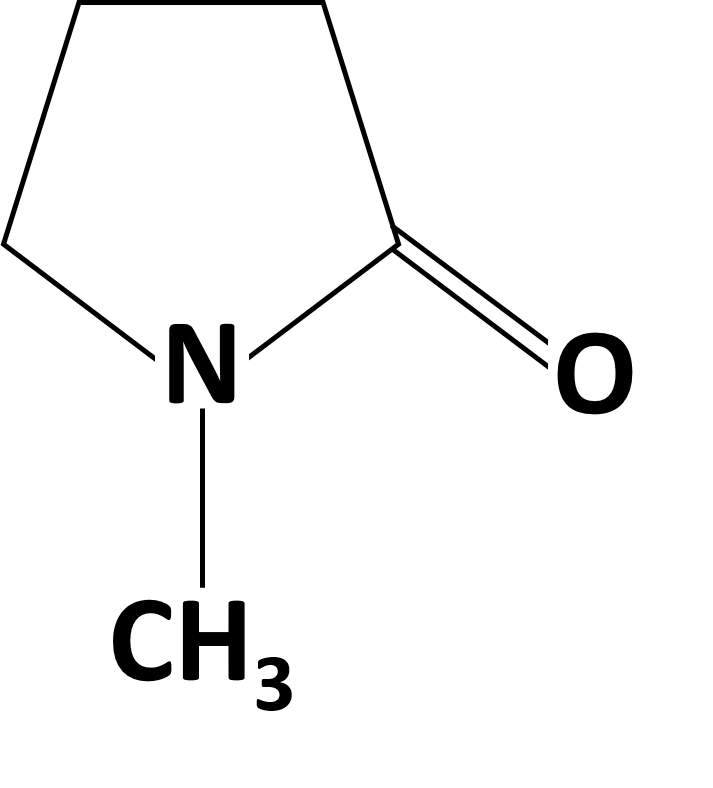
\includegraphics[width=0.75\textwidth]{Figures/chap7fig/NMP}
\caption{Structure of N-methyl pyrrolidinone, NMP.}
\label{Figures/chap7fig:NMP}
\end{figure}

\begin{table}
\caption{List of solvents used for making cathode slurries.} \label{tab1}
\begin{center}
 \begin{tabular}{|c|c|c|c|} 
 \hline
 \textbf{Solvent} & \textbf{Polarity} & \textbf{Boiling point} & \textbf{Price}\\
 \textbf{} & \textbf{} & \textbf{($^{\circ}$C)} & \textbf{(\$L$^{-1}$)}\\
 \hline
 \hline
IPA & 0.55 & 82 & 83 \\
Toluene & 0.09 & 110 & 88 \\
Acetone & 0.35 & 56 & 93 \\
Methanol & 0.76 & 65 & 112 \\ 
Butanol & 0.59 & 117 & 143 \\
DMSO & 0.44 & 189 & 198 \\
DMF & 0.39 & 153 & 207 \\
DMA & 0.35 & 165 & 211 \\
Acetonitrile & 0.35 & 82 & 221 \\
NMP & 0.35 & 202 & 259 \\
 \hline
\end{tabular}
\end{center}
\end{table}

\section{Experimental methods}
NMP/PVDF mixtures were made by dissolving 18 mg of PVDF in 1.25 ml of anhydrous NMP. A given amount of SPCB and active material was dispersed in the PVDF/NMP solution to meet the desired active material:SPCB::PVDF ratios. To ensure the thorough mixing of the SPCB particles into the polymer solution, the solution was stirred overnight. Electrode laminates were prepared by casting the slurries onto a metal foil by the doctor blade method. All the electrode films had approximately the same loading of active material (around 5-6 mg cm$^{-2}$) to eliminate the thickness effect on the electrochemical performance of the electrode. After coating the foils, the laminates were dried at 80$^{\circ}$C for two hours and then at 120$^{\circ}$C for 12 hours under vacuum. It is essential that the solvent completely evaporates and is removed from the coated electrode. It was noted that DMSO/PVDF, DMF/PVDF, DMA/PVDF and NMP/PVDF mixtures resulted in clear solutions, while ethanol, isopropanol, toluene, acetone, methanol and butanol had a cloudy appearance. 
In addition, the boiling point of the solvents was a limiting factor. High volatility of the solvents resulted in quick drying of the slurries. Cathodes that used low boiling points such as acetone, ethanol, methanol isopropanol and acetonitrile, developed cracks on their surface due to high evaporation rates, which rapid drying of the coating before they were vacuum dried.
Slurries that used DMSO, DMF, DMA, NMP, butanol and toluene as solvents yielded crack-free coatings. Consequently, the cathodes that were used for electrochemical tests were the ones made from DMSO, DMF and DMA.
The cathodes were tested via galvanostatic charge/discharge cycles in Figure \ref{Figures/chap7fig:hBNsolvents}. Same active material was used for all the cells, which is why the discharge capacities did not vary a lot. Figure \ref{Figures/chap7fig:hBNsolvents}b  shows that overall capacity of DMA based cathode was highest in its first cycle. However, it also recorded the fastest capacity fading. A possible explanation could be deducted from the coulombic efficiencies shown in Figure \ref{Figures/chap7fig:hBNsolventsCE}b. With efficiencies higher than 100\% for almost every cycle, it is likely that a few side reactions took place. DMSO-based cathodes showed consistent but high cell efficiencies >100\% (Figure \ref{Figures/chap7fig:hBNsolventsCE}a). 

\begin{figure}[tbh!]
\centering
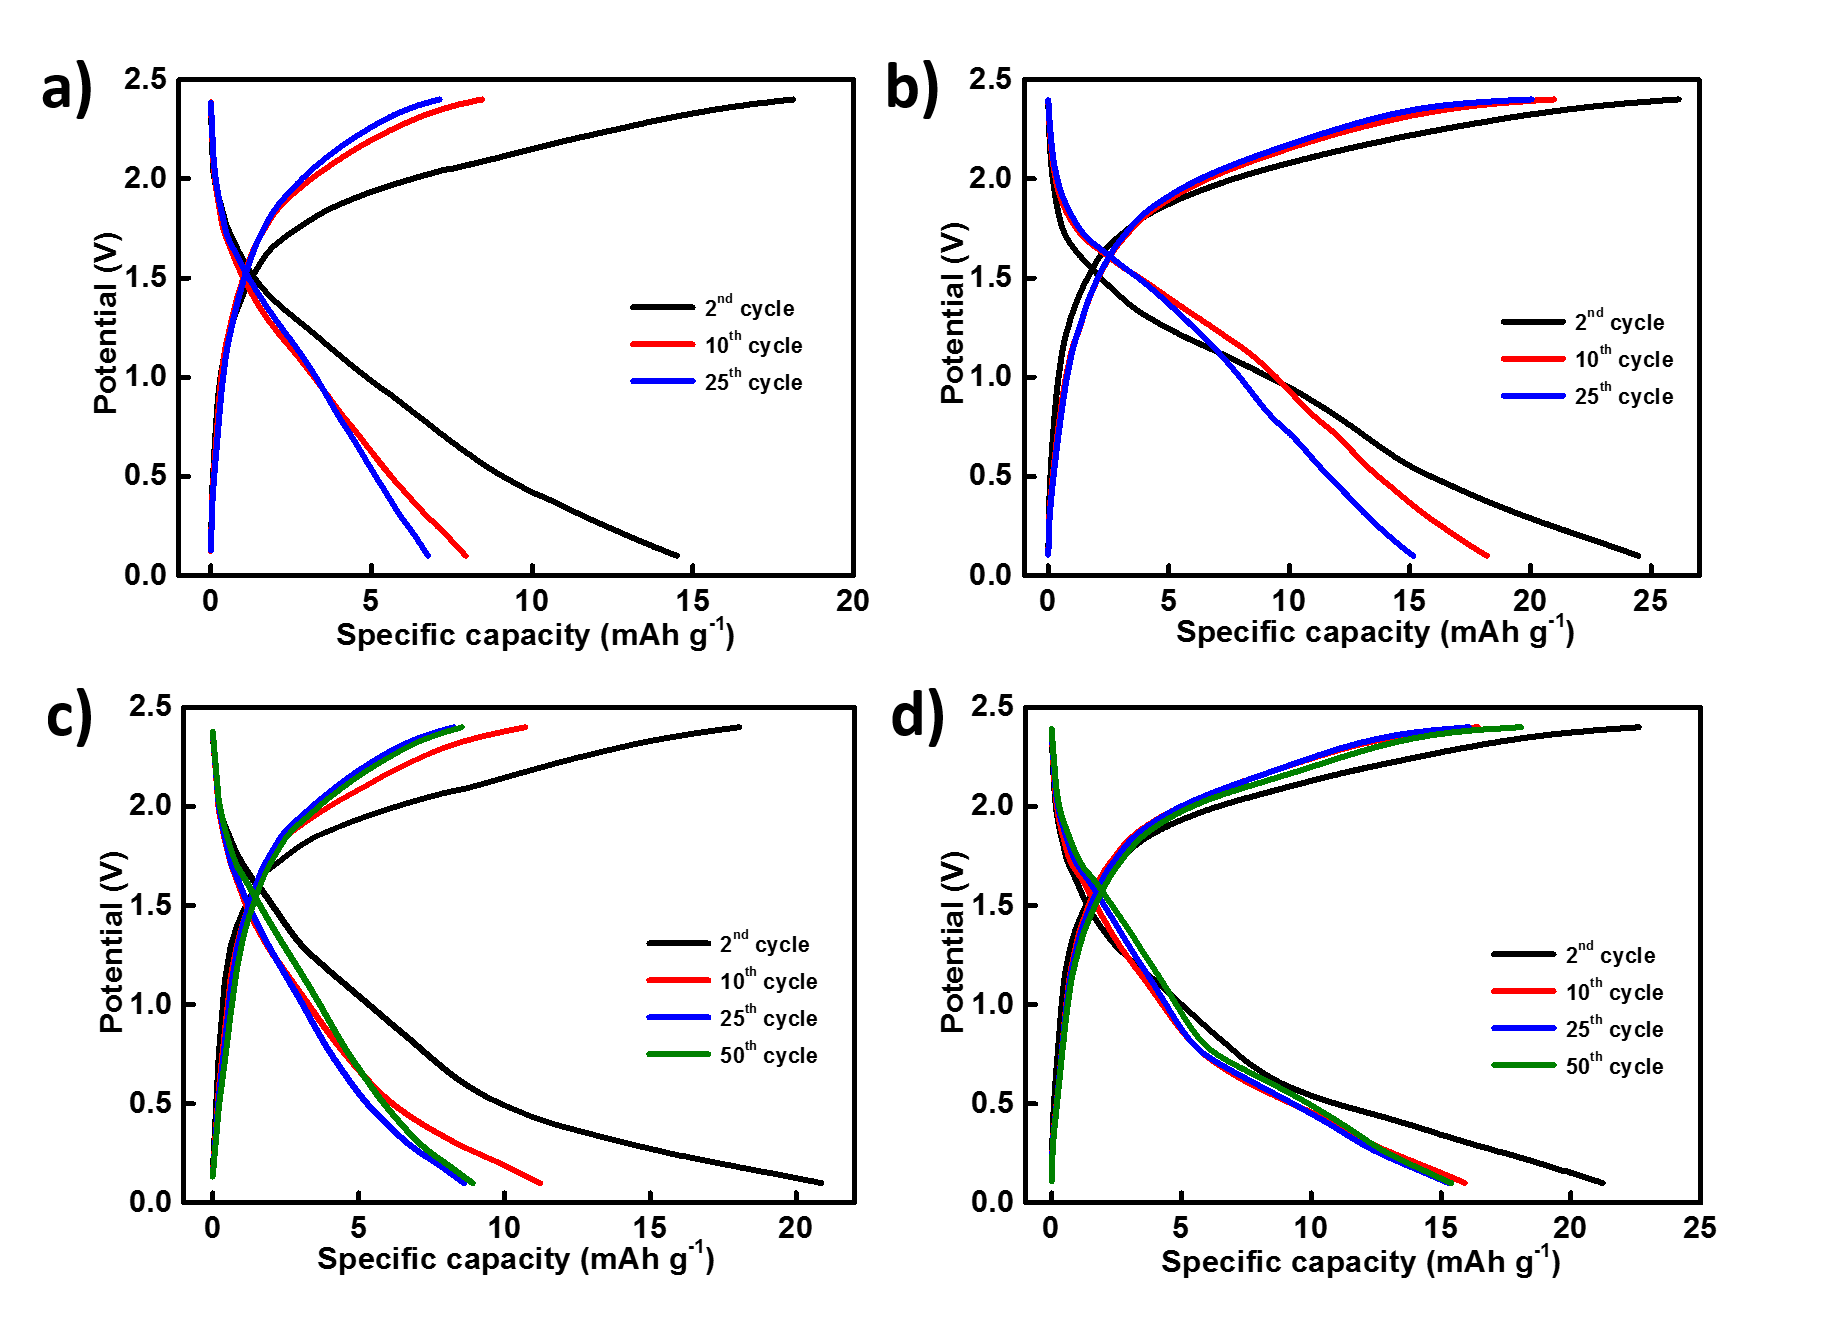
\includegraphics[width=\textwidth]{Figures/chap7fig/hBNsolvents}
\caption{Galvanostatic charge and discharge curves of aluminium-ion cells using different solvents, a) DMSO, b) DMA, c) DMF and d) NMP.}
\label{Figures/chap7fig:hBNsolvents}
\end{figure}

\begin{figure}[tbh!]
\centering
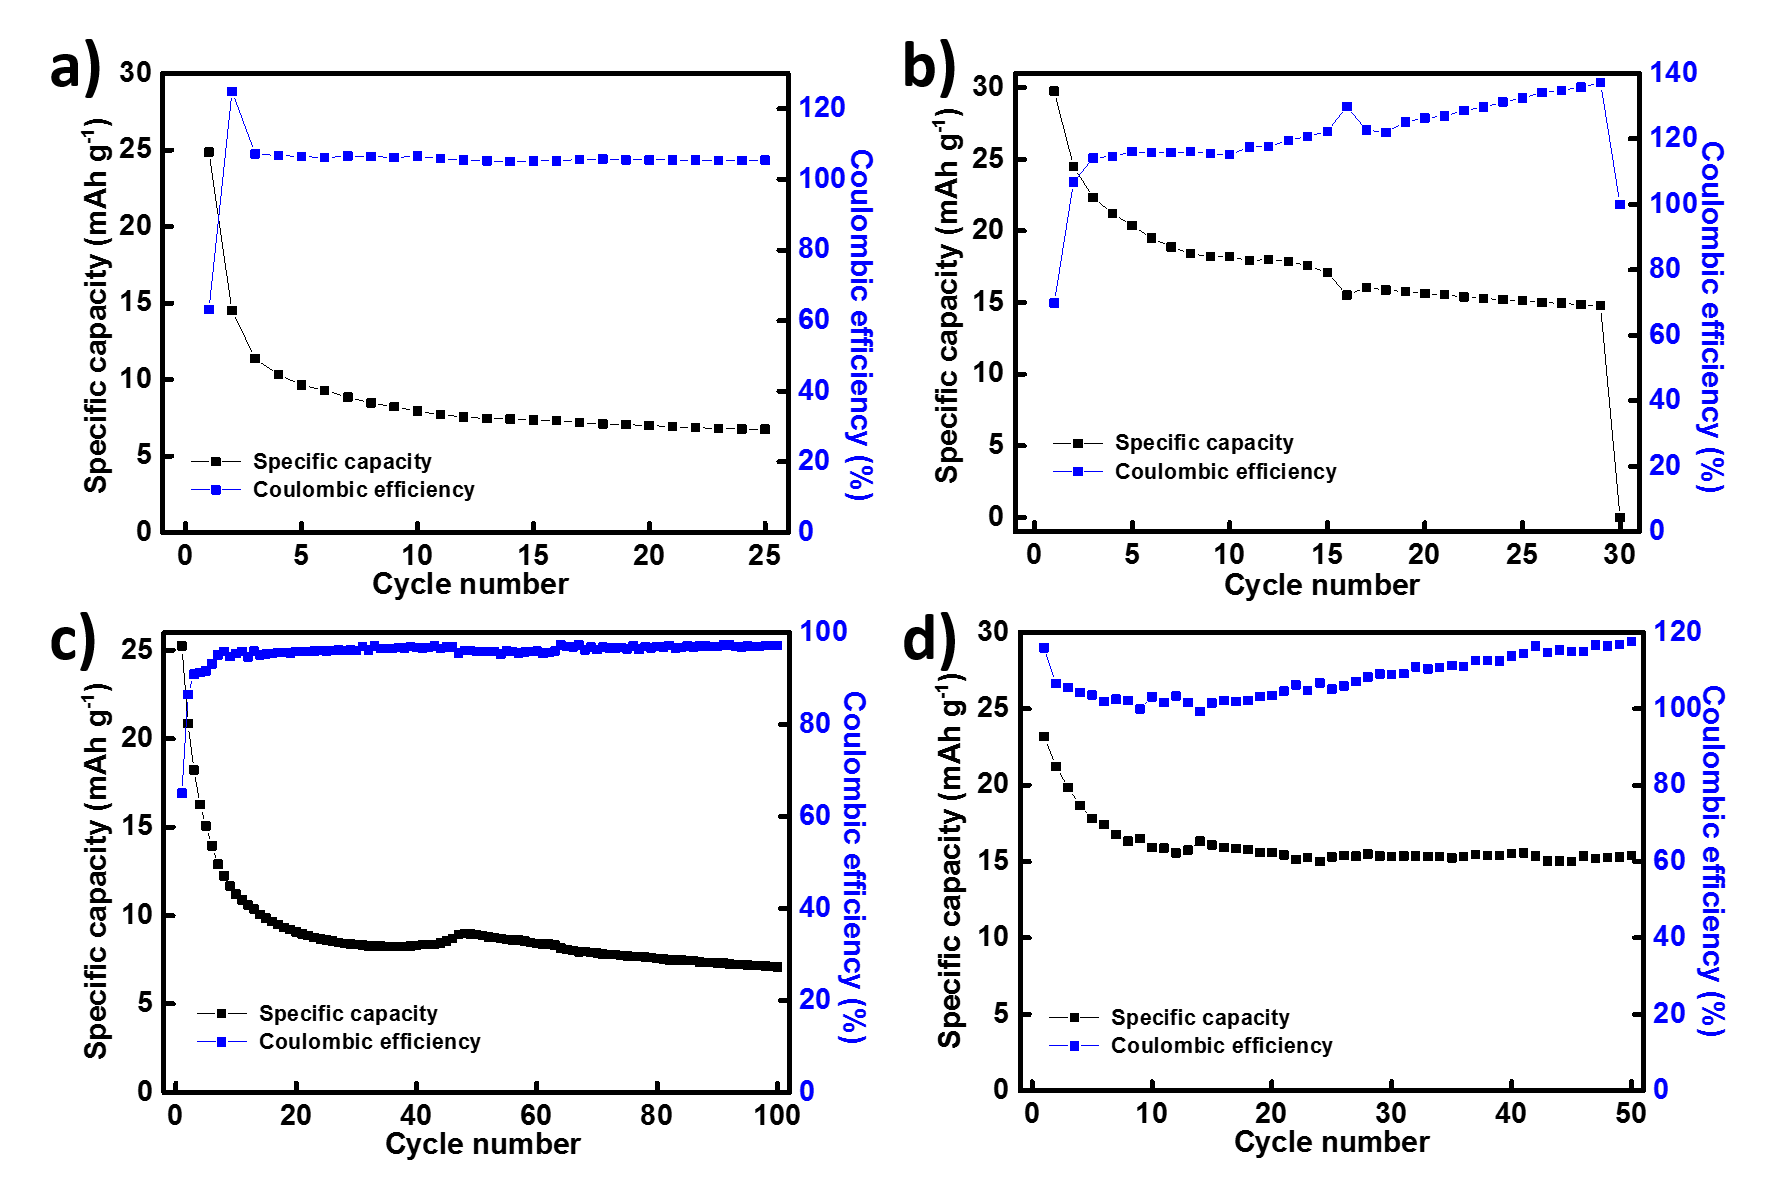
\includegraphics[width=\textwidth]{Figures/chap7fig/hBNsolventsCE}
\caption{Performance of aluminium-ion cells using different solvents, a) DMSO, b) DMA, c) DMF and d) NMP.}
\label{Figures/chap7fig:hBNsolventsCE}
\end{figure}

Figure \ref{Figures/chap7fig:hBNsolvents}c showed that with increasing cycle numbers, capacity of DMF-based cathode decreased faster than NMP based cathode, Figure \ref{Figures/chap7fig:hBNsolvents}d. Though, cell efficiency for DMF (98\%), Figure \ref{Figures/chap7fig:hBNsolventsCE}c, was better than that for NMP-based cathode (>100\%), Figure \ref{Figures/chap7fig:hBNsolventsCE}d.

\begin{figure}[h!]
\centering
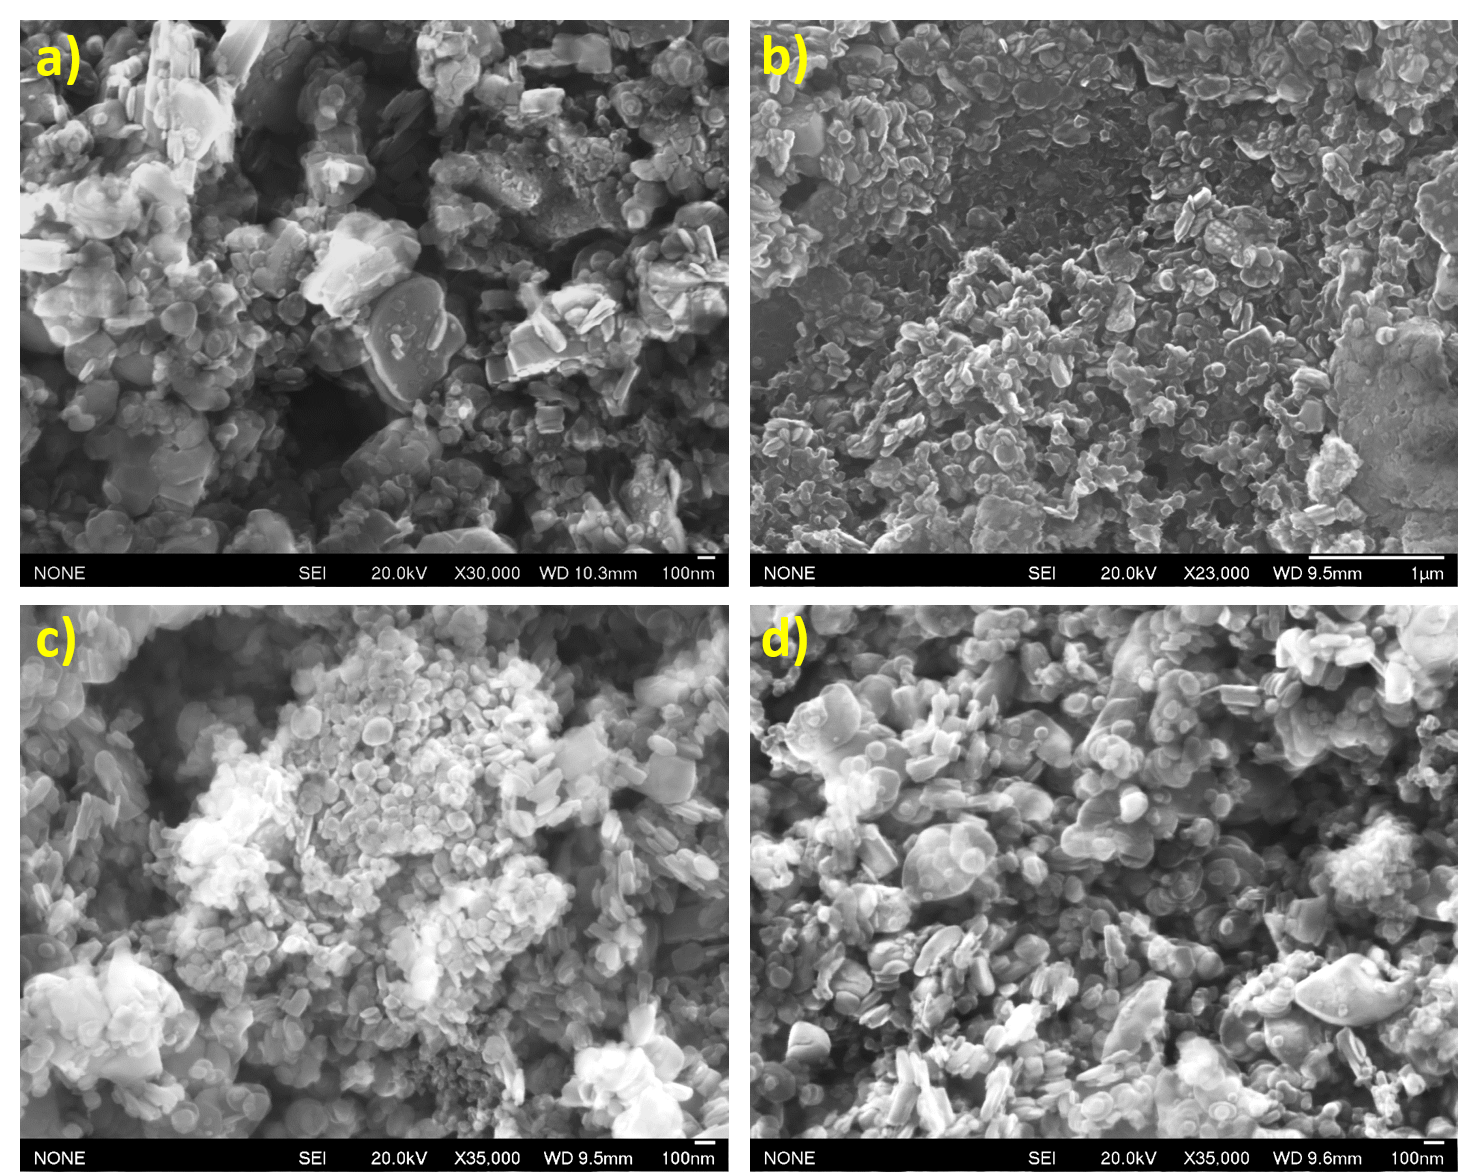
\includegraphics[width=\textwidth]{Figures/chap7fig/hBNsolventSEM}
\caption{Scanning electron microscopic images of pristine cathodes using a) DMSO, b) DMA, c) DMF and d) NMP as solvents.}
\label{Figures/chap7fig:hBNsolventSEM}
\end{figure}

Figure \ref{Figures/chap7fig:hBNsolventSEM} shows the SEM images. With DMSO and DMA, the electrode is shown to be a stack of active material, Figure \ref{Figures/chap7fig:hBNsolventSEM} a and b. SPCB agglomerates are not homogeneously dispersed in the electrode, since these particles easily flocculate as a result of their large surface area. DMF and NMP-based cathodes appeared evenly distributed and seemed to be immersed into a matrix of PVDF and SPCB composite, Figure \ref{Figures/chap7fig:hBNsolvents} c and d.\\
Overall, DMF-based cathodes maintained their specific discharge capacity after 50 cycles, with a very high coulombic efficiency $\sim$ 100\%. It seems DMF can be alternatively used as an electrode solvent, which would reduce the battery production costs. 

\subsection*{Current collectors}

\begin{table}
\caption{List of materials used as current collectors in increasing order of their marker price.} \label{t2}
\begin{center}
 \begin{tabular}{|c|c|c|c|} 
 \hline
 \textbf{Material} & \textbf{Thickness} & \textbf{Price} & \textbf{Conductivity} \\
 \textbf{Material} & \textbf{(mm)} & \textbf{(\$)} & {X 10$^{7}$}({$\Omega$}m)$^{-1}$ \\
  \hline
 \hline
Steel & 0.1 & 1.0 & 0.6 \\ 
Carbon paper & <0.1 & 1.2 & 6.5 \\
Aluminium & 0.1 & 3.04 & 3.6 \\
Brass & 1 & 5.07 & 1.4 \\
Copper & 0.1 & 9.91 & 5.9 \\ 
Nickel foam & 1 & 17.93 & 1.4 \\
Molybdenum & 0.1 & 39.61 & 1.9 \\
\hline
\end{tabular}
\end{center}
\end{table}

A current collector is a conductive solid connected to the electrode with external loading. The primary role of a current collector is to provide support to the electrodes (cathode and/or anode), collect the accumulated electrical energy from the electrode. A common current collector is a metal foil onto which a slurry is coated. A good connection between the active material and the metal foil is established only after a slow drying process which evaporates the solvent and binds it to the CC. Many metal foils have been used as metal/alloys foils in LIBs, such as nickel, copper, aluminium and steel. LIBs use two metal foils. Copper is used for the anode and aluminium is used for the cathode. This is because the two metal foils are stable at different potentials. Copper is electrochemically stable at a lower potential--
 V vs. Li\ce{Li+}, whereas aluminium is stable at a higher potential-1.34 V vs. Li\ce{Li+}. Aluminium cannot be used in our setup because it acts an anode and any contact between the active material and the anode would create a short circuit.  A CC should allow a stable flow of electrons, and should be ionically insulated. A good CC should be mechanically robust, and freestanding (usually with a macroscale size). Since a CC should be electrochemically inert, we could not use nickel foil because it oxidised at 1.1 V vs. Al/\ce{Al3+}. Steel, which is light in weight and cheap, underwent a vigorous reaction with our electrolyte and resulted in undesirable products, which resulted in rapid capacity decay and a very short cycle life. It seemed that \ce{AlCl3}/EmImCl corroded in presence of steel as can be seen in Figure \ref{Figures/chap7fig:steeleffect}. To avoid this, a CC should be within the electrochemical window if the electrolyte being used. Chemical potential of a CC ({$\mu${${_{cc}}$}} < 2.5 V) vs. Al/\ce{Al$^{3+}$}. Molybdenum foil ticked all the boxes and therefore was chosen as the CC in all our battery tests.  
 We compared the cell performances of all cells using different CCs, showed in Figure \ref{Figures/chap7fig:hBNCCCDC}. Firstly, carbon as a CC stands out from the other CCs. The cell recorded the highest discharge capacity at 82 mAh g$^{-1}$ (in green). When run for longer, the capacity was retained at 70 mAh g$^{-1}$ after25 cycles. The curve was exceptionally similar to the CDCs of an Al/graphite cell (inset Figure \ref{Figures/chap7fig:hBNCCCDC}b). This lead us to the conclusion that hBN became dormant in this cell and graphitic nature of the carbon paper took over and acted as the active material intercalating the \ce{AlCl4-} ions during charge. Steel, nickel, copper, brass and copper foils did not allow any charge or discharge to take place. Despite applying a continuous current, the charges seemed to accumulate and provided an unstable flow of electrons. Copper is a highly conductive metal; when aluminium electroplates, a few ions might get deposited on the CC creating a short circuit. Steel on the other hand contains chromium, which reacts with \ce{AlCl3}/EmImCl and some greenish stuff can be observed after we open the cell Figure \ref{Figures/chap7fig:steeleffect} \cite{reed_roles_2013}. This confirms that a side reaction took place, which consumed the electrolyte. Brass is less conductive than copper, as seen in Table \ref{t2}, and it contains other metals which have impeded the cell reaction and its capacity.   
%The battery performance results are shown in figure 6. It can be seen that the charging behaviour of brass, copper and aluminium have a similar tendency. Starting from different voltages, charging the system does not result in an actual increase in voltage, thus charge built-up as desired. As shown in figure 6 a), brass, copper and aluminium tend to reach a specific equilibrium voltage regardless of the energy provided to the system. Energy consumption without any charging indicates other processes being present consuming the provided energy. It is assumed that the energy consumed is used to disintegrate the substrate material. Ideally, the substrate is not in direct contact with the electrolyte. In reality however there will always be some sort of contact area present. The Al atoms in the aluminium and eventually the iron or chromium atoms present in the brass and copper are resulting in the disintegration of the substrates as such. As a reference how a single charging/discharging cycle should appear, figure 6 b)	shows a complete cycle for a BN RAB using a molybdenum substrate. Here the desired charge built-up can be observed until reaching the cut-off limit of 2.4V and the following discharging can be observed. A very unique charging behaviour could be observed for carbon coated aluminium as a substrate for the hBN slurry as shown in figure 6 c). A mixture of fast charging and abrupt rapid discharging can be observed. Knowing the tendency of the aluminium shown in figure 6 a) to completely discharge to the cutoff voltage of 0.1, it can be assumed that the rapid discharging behaviour results from the underlying aluminium. As discussed in section 2, carbon based RAB have been shown to work well and achieve high charging rates. Therefore it is assumed that the charging phases are either caused by the BN cathode material or by the underlying carbon coating. Even though the just discussed tested alternatives did not succeed in charging at all, Ni foam and Carbon paper did successfully charge and discharge. The corresponding capacities are shown in figure 6 d). The fact that the capacity of the battery with Ni foam as substrate is noticeable lower is caused by the fact that nickel oxidises at voltages exceeding 0.9 V. This relatively low cutoff voltage is one reason why the capacity is rather low. It can be noticed that carbon paper as a substrate has a very high capacity. Comparing the achieved result however with results previously achieved by researchers of the VUW using carbon paper only, showed that that the overall performances are very much alike. This leads to the conclusion, that contrary to the desired hBN, mainly the carbon paper participated in the intercalation/deintercalation process. Therefore it is not a suitable substrate candidate for the specific use in the hBN based batteries due to the ions preferred affinity towards the carbon paper rather than to the hBN cathode material.
\begin{figure}[tbh!]
\centering
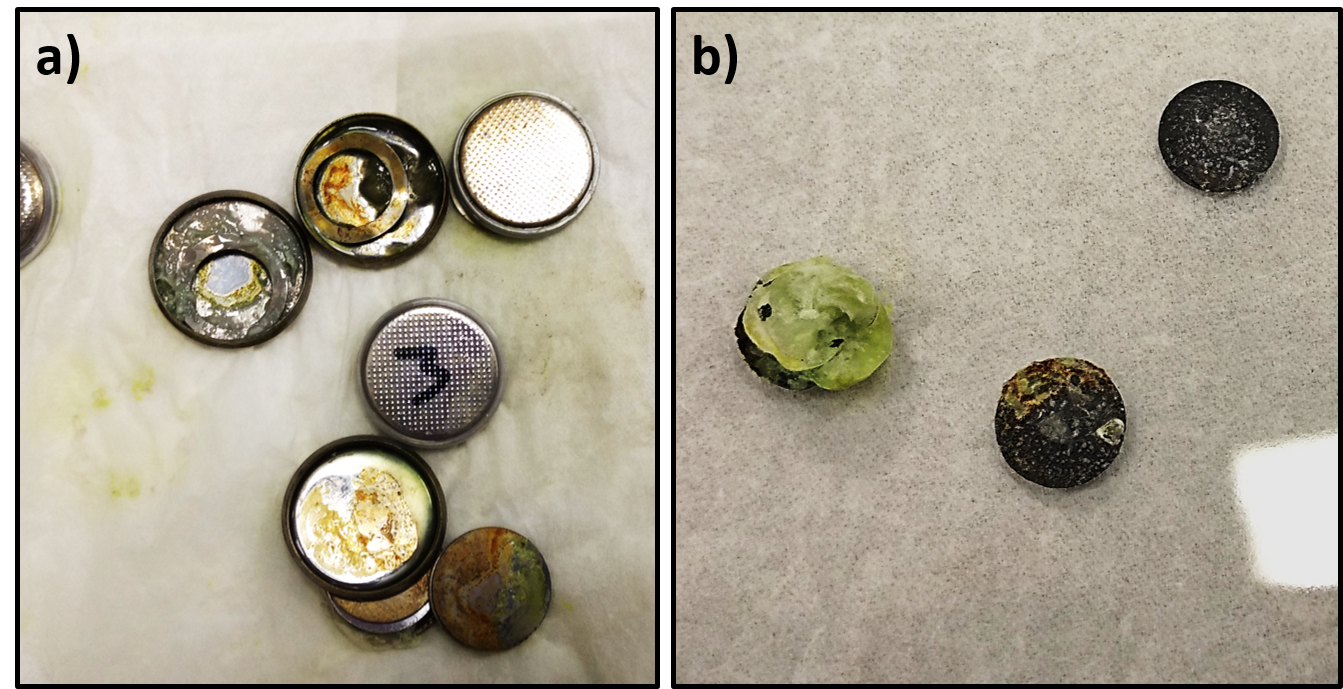
\includegraphics[width=\textwidth]{Figures/chap7fig/steeleffect}
\caption{SEM images of pristine hBN cathodes using a) DMSO, b) DMA, c) DMF and d) NMP solvents.}
\label{Figures/chap7fig:steeleffect}
\end{figure}
\begin{figure}[tbh!]
\centering
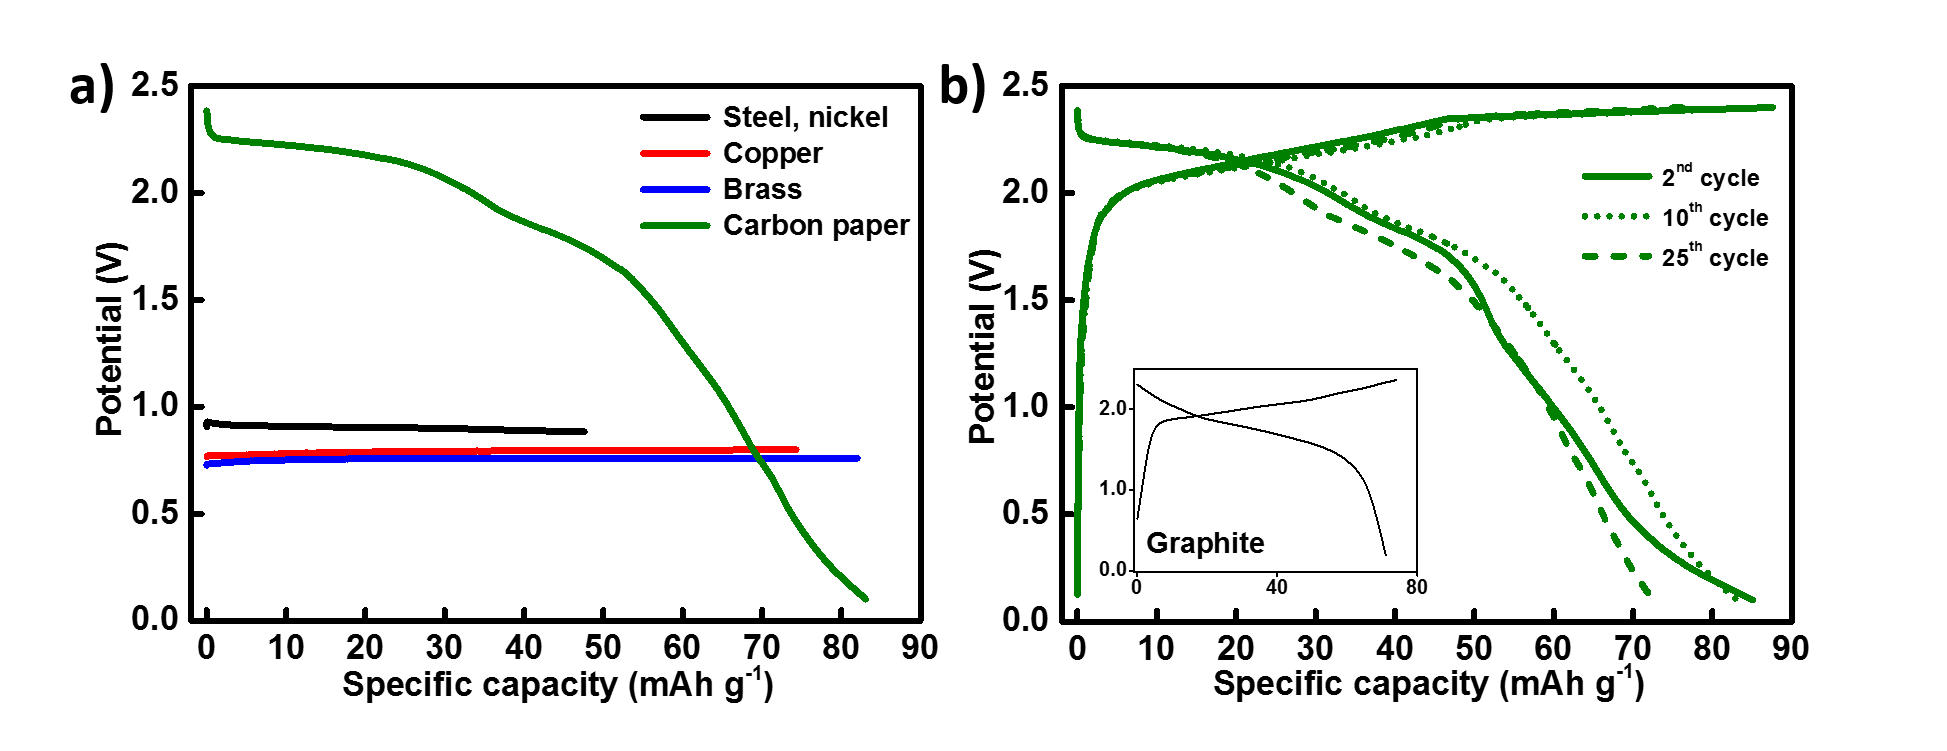
\includegraphics[width=\textwidth]{Figures/chap7fig/hBNCCCDC}
\caption{Galvanostatic cycles using hBN as the active material with a) steel and nickel foils (black), copper sheet (red), brass sheet (blue) and carbon paper (green) as current collectors in a two-electrode setup at a current rate of 40 mA g$^{-1}$. b) Performance of Al/hBN cell using carbon paper as the current collector which showed graphite dominating as active material (inset: CDC curve of an Al/graphite cell) }
\label{Figures/chap7fig:hBNCCCDC}
\end{figure}

\section{Conclusion and future outlook}
Replacing NMP with a cheaper solvent would be beneficial when commercialising AIBs. However, no solvent has proven to be as efficient as NMP yet. LIB plants recycle NMP on a regular basis. During vacuum drying process, NMP is collected from the exhaust gases and is used to clean equipment and is reused. This method can be applied while manufacturing AIBs, which would further reduce the battery production costs. 
Molybdenum, titanium and ITO turned out to be a good current collectors for our AIBs. Although a CC is inactive in a cell, however it occupies enough space- almost 9\%! If this number is reduced, the cell will record a higher energy density. One can use a thinner foil (structurally stable) instead of a thick one to attain a higher capacity value. In fact a thicker coating of the active material might seem as a solution but that limits the ion and electron transport across the electrode leading to a lower cycle life. 3D current collectors based on carbon might be the way to go. In LIBs, graphite foam has been used as a CC, since it does not intercalate at a potential >0.5V. Ruoff \textit{et al.} \cite{ji_ultrathin_2012} use graphene foam as a current collector for the first time. A 3D CC not only provides a dense interconnected structure that can rapidly transport /diffuse ions, but also an excellent conductivity. CC with a large pore volume accommodates expansion of active material would also prevent cathode pulverisation. 
